\section{Présentation de Theodo}

\subsection{Activités et croissance}

Theodo est une \textbf{startup de développement web agile} dont le but est de \textbf{résoudre efficacement les problèmes \foreignlanguage{english}{business} de ses clients}.

Elle a été fondée en 2009 par Benoît Charles-Lavauzelle et Fabrice Bernhard, tous deux diplômés de l'Ecole polytechnique et partageant une même passion pour le web. La stratégie de Theodo est de \textbf{créer un nouveau métier} qui se situe entre les ESN\footnote{\textit{Entreprise de service du numérique}, anciennement \textit{société de services en ingénierie informatique} (SSII ou SS2I).} classiques et les sociétés de conseil. L'objectif vis-à-vis des clients est donc de les conseiller dans le choix d'une solution répondant à une problématique business, mais également de développer cette solution tout en accompagnant la transformation digitale des entreprises.

Pour mener à bien cette double mission dans chacun des projets, Theodo recrute ses développeurs dans les plus grandes écoles d'ingénieur pour s'assurer d'avoir des \textbf{profils polyvalents}, à l'aise techniquement mais également capables de comprendre et de répondre aux problématiques métier des clients. Les développeurs sont accompagnés dans leur progression et l'objectif de Theodo est de former des CTO\footnote{\textit{\foreignlanguage{english}{Chief Technology Officer}}, en français \textit{directeur de la technologie}.} en cinq ans et d'accompagner ceux qui le souhaitent dans la création de leur entreprise dans le cadre de la \textit{\foreignlanguage{english}{Theodo Academy}}, la "startup studio" de Theodo.

Les résultats et la croissance de Theodo sont impressionnants : la jeune entreprise a \textbf{multiplié par 10 son chiffre d'affaires ainsi que son effectif en 4 ans} pour arriver aujourd'hui à une centaine d'employés et à 13 millions d'euros de chiffre d'affaire. La satisfaction des clients, qui est l'unique indicateur de succès de Theodo, est très importante avec un taux de "réachat" supérieur à 100\%. Ces clients sont par ailleurs d'horizons très variés et vont des startups comme LaFourchette ou BlablaCar aux grands comptes comme la BNP, la Société Générale et LVMH. Enfin, l'esprit d'équipe est très fort chez Theodo ; cela se traduit notamment par une grande satisfaction des employés : en 2015, Theodo était la deuxième startup au classement "Happy at work".

\subsection{La méthodologie de gestion de projet comme facteur clé de succès}

Une des grandes valeurs ajoutées de Theodo est de bousculer les cycles de développement classiques des produits en mettant en œuvre des \textbf{méthodes de développement dites "agiles" pour créer de la valeur très rapidement pour leurs clients}.

\subsubsection*{Qu'est-ce que l'agilité ?}

L'agilité est une \textbf{philosophie de développement de produit} qui s'oppose aux méthodes traditionnelles de telles que le modèle du cycle en V. Les rédacteurs du \textit{manifeste agile}\footnote{Le manifeste agile est disponible à l'adresse : http://agilemanifesto.org/} ont pour ambition de \textbf{réduire le \textit{time-to-market}}\footnote{C'est le temps qui sépare le début de la conception d'un produit du moment où ce produit est disponible pour ses utilisateurs.} des produits développés : amener au plus vite le produit à l'utilisateur final permet en effet d'inclure les retours utilisateurs au développement pour ajuster le produit au besoin réel des utilisateurs.

Cette \textbf{approche itérative}, par cycles de développement courts suivis d'une mise à disposition des utilisateurs, s'oppose en effet à l'approche prédictive et séquentielle du modèle du cycle en V qui souffre aujourd'hui de défauts importants :
\begin{itemize}
\item Le \textit{time-to-market} est très grand puisque les utilisateurs ne peuvent tester l'application qu'une fois celle-ci conçue, développée et testée. La valeur créée lors du développement n'est donc visible de l'utilisateur qu'à la toute fin du processus : on parle d'"effet tunnel".
\item L'utilisateur final n'est pas inclus au processus de développement : l'écart entre le besoin initial exprimé et le produit livré peut donc être très important.
\item Enfin, le produit n'est déployé\footnote{Le déploiement d'un logiciel est sa mise à disposition auprès des utilisateurs.} qu'à la toute fin : le marché ayant évolué lors du cycle de développement, il est possible que le produit livré ne soit plus du tout adapté aux utilisateurs et ne rapporte rien aux concepteurs.
\end{itemize}

\begin{figure}[!ht]
    \center
    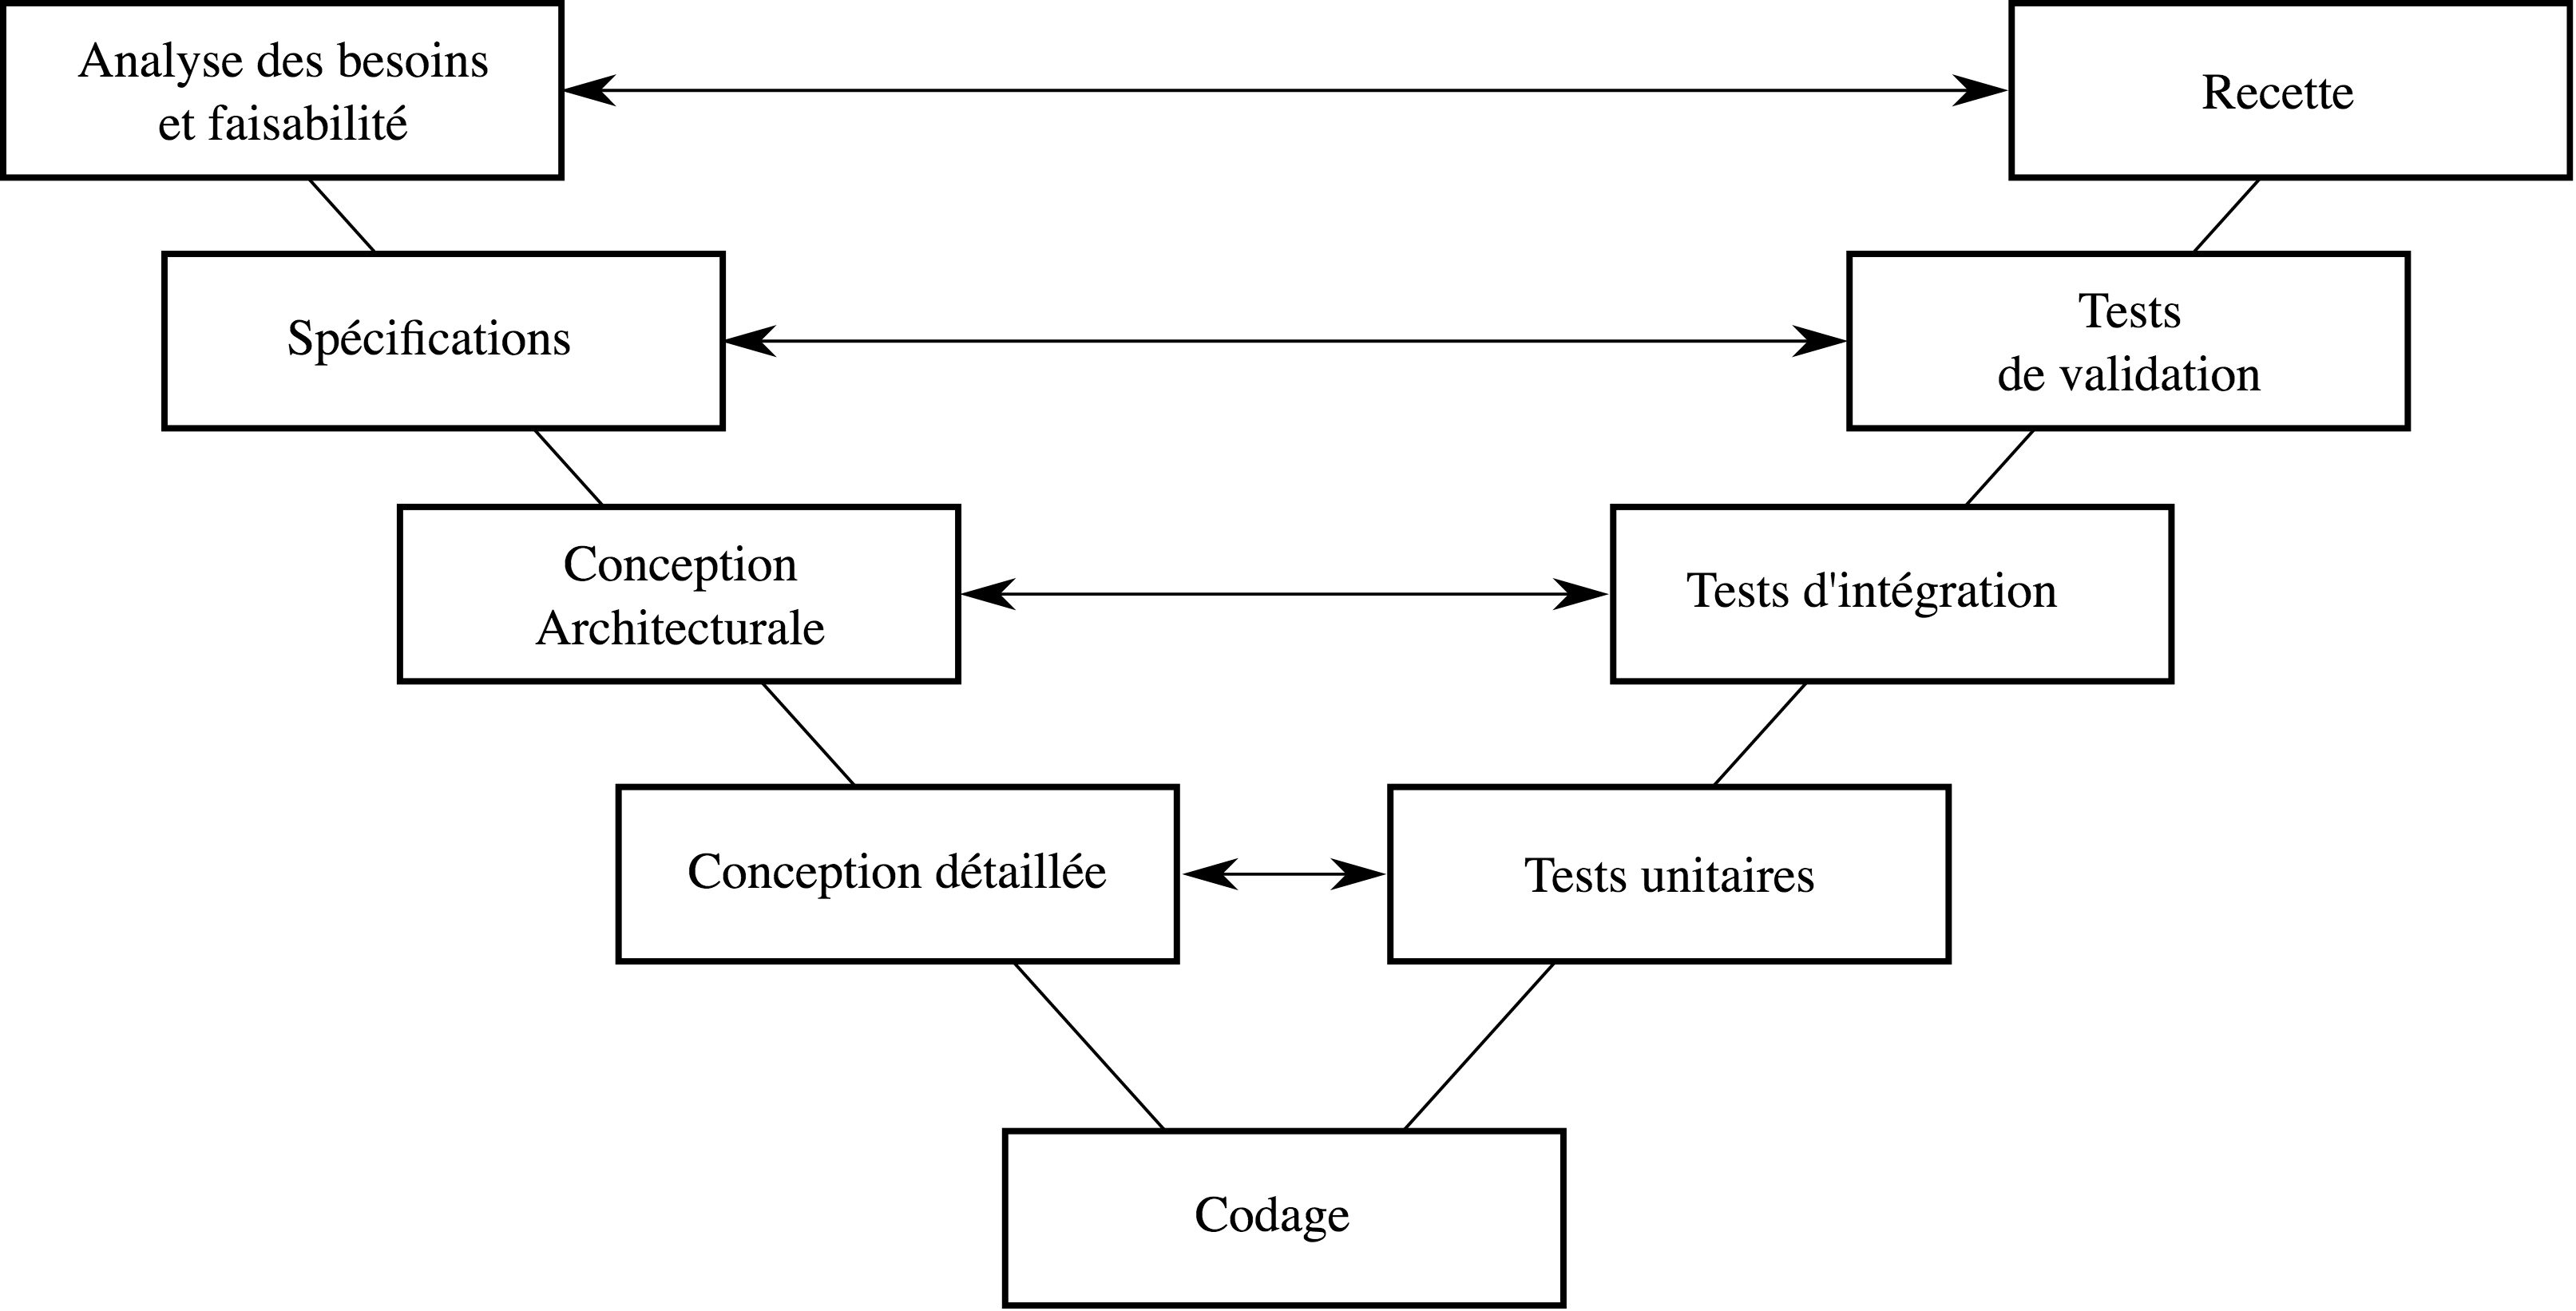
\includegraphics[width=0.8\textwidth]{./images/I_1_cycle_V.png}
    \caption{Les étapes du cycle en V [Source : wikipedia.org]}
\end{figure}

Par opposition à l'approche du cycle en V, le manifeste agile met en avant quatre valeurs essentielles en privilégiant :
\begin{itemize}
\item \textbf{Les individus et leurs interactions} plus que les processus et les outils.
\item \textbf{Du logiciel qui fonctionne} plus qu’une documentation exhaustive.
\item \textbf{La collaboration avec les clients} plus que la négociation contractuelle.
\item \textbf{L’adaptation au changement} plus que le suivi d’un plan.
\end{itemize}

Cette philosophie de développement est \textbf{particulièrement pertinente pour les marchés qui évoluent très rapidement}, et est en conséquence de plus en plus répandue dans les technologies de l'information.

\subsubsection*{La méthode Scrum appliquée chez Theodo}

Il existe plusieurs méthodes de développement de produits qui sont basées sur la philosophie agile. Chez Theodo, c'est la \textbf{méthode Scrum}\footnote{\textit{Scrum} signifie \textit{mêlée} en anglais. Ce terme provenant du rugby souligne que l'équipe projet doit avancer en étant soudée.} qui est utilisée.

La méthode Scrum part du principe qu'un projet de développement ne peut être entièrement planifié à l'avance. Un projet est donc découpé en des itérations successives de durée fixe - une semaine chez Theodo - appelées \textbf{Sprints}. Les Sprints permettent à l'équipe de développement de se concentrer sur un nombre limité de \textbf{fonctionnalités identifiées comme prioritaires} sur une durée très courte, et donc de \textbf{créer de la valeur efficacement et rapidement}.

Une équipe projet Scrum est auto-organisée et ne possède pas de chef de produit au sens strict du terme. On trouve dans cette équipe :
\begin{itemize}
\item \textbf{Le propriétaire du produit}, ou \textbf{\textit{Product Owner}} représente le client et les utilisateurs. C'est lui qui est chargé de prioriser les fonctionnalités du \textit{product backlog}\footnote{Le \textit{product backlog}, ou carnet de produit, est l'ensemble des fonctionnalités à implémenter dans le produit final.} et de fixer les objectifs du Sprint au début de celui-ci.
\item \textbf{Le Scrum Master}, ou \textbf{\textit{facilitateur}} s'assure que la méthode est comprise et appliquée par l'équipe.
\item \textbf{Un ou plusieurs développeurs}, dont le rôle est de développer et de délivrer les fonctionnalités prévues en début de Sprint.
\end{itemize}

A l'issue de chaque Sprint, l'équipe réunit pour mettre à jour et reprioriser le \textit{product backlog}, en se basant notamment sur les retours des utilisateurs. Pour que ces derniers soient fréquents et utilisables, Theodo pratique le \textbf{déploiement continu} afin qu'une mise en production de l'application soit effectuée au moins toutes les deux semaines.

\subsection{Organisation de l'entreprise}

Chez Theodo, le principe d'organisation est très simple : pour que tout le monde pousse l'entreprise dans la même direction, \textbf{chacun doit faire partie d'une équipe projet}. De cette manière, tous les employés mettent la méthodologie en pratique au quotidien et peuvent créer de la valeur pour Theodo et pour leurs clients. Même le CEO\footnote{\textit{\foreignlanguage{english}{Chief Executive Officer}}, en français \textit{directeur général}.} et le CTO sont staffés sur des projets !

En conséquence, l'entreprise adopte une \textbf{organisation "à plat"} dans laquelle les tâches de chacun ne sont pas définies par une hiérarchie précise, mais par les projets en cours et les rôles éventuels - voir plus bas. Surtout, pour pouvoir assurer un double service de conseil et de développement auprès de ses clients, Theodo ne compte que deux "profils" d'employés :
\begin{itemize}
\item Les \textit{ingénieurs-développeurs}
\item Les \textit{\foreignlanguage{english}{business developers}}
\end{itemize}

Ce sont à partir de ces deux profils que les équipes projet sont constituées : les développeurs forment l'équipe technique alors que le Scrum Master et le commercial sont des \textit{\foreignlanguage{english}{business developers}}. Les employés sont donc regroupés par équipe projet au sein de l'open space et se déplacent dès qu'ils en changent.

Certains employés obtiennent des rôles qui s'ajoutent à leurs projets dès lors qu'ils ont assez progressé au sein de l'entreprise. Chez les \textit{\foreignlanguage{english}{business developers}} :
\begin{itemize}
\item Les administrateurs financiers ont pour rôle de gérer les finances de l'entreprise
\item Les membres de l'équipe \textit{\foreignlanguage{english}{sales}} trouvent des nouveaux projets en prospectant parmi les clients potentiels
\item Les membres de l'équipe \textit{\foreignlanguage{english}{Joinus}} sont chargés du recrutement
\end{itemize}

Chez les développeurs, les \textbf{architectes} sont des développeurs expérimentés qui sont compétents pour réaliser les challenges techniques de leurs projets\footnote{La challenge technique est le moment du choix de la solution technique la plus adaptée au problème \foreignlanguage{english}{business} du client. C'est aussi à ce moment là que les outils de développement - langage et \foreignlanguage{english}{framework} - sont fixés.}. Ils sont staffés sur plusieurs projets simultanément - trois au maximum - et apportent leur expérience pour s'assurer que les projets réussissent ; ils sont des éléments très importants pour la progression de Theodo et la qualité des produits développés.

Un des éléments moteurs de la progression chez Theodo est le \textbf{système de coachs et de coachés}. Chacun a un coach parmi les employés expérimentés, vers lequel il peut se tourner dès qu'il a un doute ou un problème : ce geste s'appelle le \textbf{\textit{andon}}\footnote{Ce terme, issu du système de production Toyota, désigne initialement un signal lumineux qui indique qu'un poste de travail rencontre un problème, provoquant une interruption partielle de la chaîne de production et la résolution immédiate du problème.}.
